\documentclass[]{article}
\usepackage{lmodern}
\usepackage{amssymb,amsmath}
\usepackage{ifxetex,ifluatex}
\usepackage{fixltx2e} % provides \textsubscript
\ifnum 0\ifxetex 1\fi\ifluatex 1\fi=0 % if pdftex
  \usepackage[T1]{fontenc}
  \usepackage[utf8]{inputenc}
\else % if luatex or xelatex
  \ifxetex
    \usepackage{mathspec}
  \else
    \usepackage{fontspec}
  \fi
  \defaultfontfeatures{Ligatures=TeX,Scale=MatchLowercase}
\fi
% use upquote if available, for straight quotes in verbatim environments
\IfFileExists{upquote.sty}{\usepackage{upquote}}{}
% use microtype if available
\IfFileExists{microtype.sty}{%
\usepackage{microtype}
\UseMicrotypeSet[protrusion]{basicmath} % disable protrusion for tt fonts
}{}
\usepackage[margin=1in]{geometry}
\usepackage{hyperref}
\hypersetup{unicode=true,
            pdftitle={DATA 606 - Homework 3},
            pdfauthor={Joshua Sturm},
            pdfborder={0 0 0},
            breaklinks=true}
\urlstyle{same}  % don't use monospace font for urls
\usepackage{color}
\usepackage{fancyvrb}
\newcommand{\VerbBar}{|}
\newcommand{\VERB}{\Verb[commandchars=\\\{\}]}
\DefineVerbatimEnvironment{Highlighting}{Verbatim}{commandchars=\\\{\}}
% Add ',fontsize=\small' for more characters per line
\usepackage{framed}
\definecolor{shadecolor}{RGB}{248,248,248}
\newenvironment{Shaded}{\begin{snugshade}}{\end{snugshade}}
\newcommand{\KeywordTok}[1]{\textcolor[rgb]{0.13,0.29,0.53}{\textbf{{#1}}}}
\newcommand{\DataTypeTok}[1]{\textcolor[rgb]{0.13,0.29,0.53}{{#1}}}
\newcommand{\DecValTok}[1]{\textcolor[rgb]{0.00,0.00,0.81}{{#1}}}
\newcommand{\BaseNTok}[1]{\textcolor[rgb]{0.00,0.00,0.81}{{#1}}}
\newcommand{\FloatTok}[1]{\textcolor[rgb]{0.00,0.00,0.81}{{#1}}}
\newcommand{\ConstantTok}[1]{\textcolor[rgb]{0.00,0.00,0.00}{{#1}}}
\newcommand{\CharTok}[1]{\textcolor[rgb]{0.31,0.60,0.02}{{#1}}}
\newcommand{\SpecialCharTok}[1]{\textcolor[rgb]{0.00,0.00,0.00}{{#1}}}
\newcommand{\StringTok}[1]{\textcolor[rgb]{0.31,0.60,0.02}{{#1}}}
\newcommand{\VerbatimStringTok}[1]{\textcolor[rgb]{0.31,0.60,0.02}{{#1}}}
\newcommand{\SpecialStringTok}[1]{\textcolor[rgb]{0.31,0.60,0.02}{{#1}}}
\newcommand{\ImportTok}[1]{{#1}}
\newcommand{\CommentTok}[1]{\textcolor[rgb]{0.56,0.35,0.01}{\textit{{#1}}}}
\newcommand{\DocumentationTok}[1]{\textcolor[rgb]{0.56,0.35,0.01}{\textbf{\textit{{#1}}}}}
\newcommand{\AnnotationTok}[1]{\textcolor[rgb]{0.56,0.35,0.01}{\textbf{\textit{{#1}}}}}
\newcommand{\CommentVarTok}[1]{\textcolor[rgb]{0.56,0.35,0.01}{\textbf{\textit{{#1}}}}}
\newcommand{\OtherTok}[1]{\textcolor[rgb]{0.56,0.35,0.01}{{#1}}}
\newcommand{\FunctionTok}[1]{\textcolor[rgb]{0.00,0.00,0.00}{{#1}}}
\newcommand{\VariableTok}[1]{\textcolor[rgb]{0.00,0.00,0.00}{{#1}}}
\newcommand{\ControlFlowTok}[1]{\textcolor[rgb]{0.13,0.29,0.53}{\textbf{{#1}}}}
\newcommand{\OperatorTok}[1]{\textcolor[rgb]{0.81,0.36,0.00}{\textbf{{#1}}}}
\newcommand{\BuiltInTok}[1]{{#1}}
\newcommand{\ExtensionTok}[1]{{#1}}
\newcommand{\PreprocessorTok}[1]{\textcolor[rgb]{0.56,0.35,0.01}{\textit{{#1}}}}
\newcommand{\AttributeTok}[1]{\textcolor[rgb]{0.77,0.63,0.00}{{#1}}}
\newcommand{\RegionMarkerTok}[1]{{#1}}
\newcommand{\InformationTok}[1]{\textcolor[rgb]{0.56,0.35,0.01}{\textbf{\textit{{#1}}}}}
\newcommand{\WarningTok}[1]{\textcolor[rgb]{0.56,0.35,0.01}{\textbf{\textit{{#1}}}}}
\newcommand{\AlertTok}[1]{\textcolor[rgb]{0.94,0.16,0.16}{{#1}}}
\newcommand{\ErrorTok}[1]{\textcolor[rgb]{0.64,0.00,0.00}{\textbf{{#1}}}}
\newcommand{\NormalTok}[1]{{#1}}
\usepackage{graphicx,grffile}
\makeatletter
\def\maxwidth{\ifdim\Gin@nat@width>\linewidth\linewidth\else\Gin@nat@width\fi}
\def\maxheight{\ifdim\Gin@nat@height>\textheight\textheight\else\Gin@nat@height\fi}
\makeatother
% Scale images if necessary, so that they will not overflow the page
% margins by default, and it is still possible to overwrite the defaults
% using explicit options in \includegraphics[width, height, ...]{}
\setkeys{Gin}{width=\maxwidth,height=\maxheight,keepaspectratio}
\IfFileExists{parskip.sty}{%
\usepackage{parskip}
}{% else
\setlength{\parindent}{0pt}
\setlength{\parskip}{6pt plus 2pt minus 1pt}
}
\setlength{\emergencystretch}{3em}  % prevent overfull lines
\providecommand{\tightlist}{%
  \setlength{\itemsep}{0pt}\setlength{\parskip}{0pt}}
\setcounter{secnumdepth}{0}
% Redefines (sub)paragraphs to behave more like sections
\ifx\paragraph\undefined\else
\let\oldparagraph\paragraph
\renewcommand{\paragraph}[1]{\oldparagraph{#1}\mbox{}}
\fi
\ifx\subparagraph\undefined\else
\let\oldsubparagraph\subparagraph
\renewcommand{\subparagraph}[1]{\oldsubparagraph{#1}\mbox{}}
\fi

%%% Use protect on footnotes to avoid problems with footnotes in titles
\let\rmarkdownfootnote\footnote%
\def\footnote{\protect\rmarkdownfootnote}

%%% Change title format to be more compact
\usepackage{titling}

% Create subtitle command for use in maketitle
\newcommand{\subtitle}[1]{
  \posttitle{
    \begin{center}\large#1\end{center}
    }
}

\setlength{\droptitle}{-2em}
  \title{DATA 606 - Homework 3}
  \pretitle{\vspace{\droptitle}\centering\huge}
  \posttitle{\par}
  \author{Joshua Sturm}
  \preauthor{\centering\large\emph}
  \postauthor{\par}
  \predate{\centering\large\emph}
  \postdate{\par}
  \date{09/11/2017}


\begin{document}
\maketitle

{
\setcounter{tocdepth}{2}
\tableofcontents
}
\subsection{3.2 Area under the curve, Part
II.}\label{area-under-the-curve-part-ii.}

What percent of a standard normal distribution
\(N(\mu = 0, \sigma = 1)\) is found in each region? Be sure to draw a
graph.\\
(a)
\(Z > -1.13 \qquad (b) Z < 0.18 \qquad (c) Z > 8 \qquad (d) |Z| < 0.5\).

\begin{enumerate}
\def\labelenumi{(\alph{enumi})}
\tightlist
\item
  \(Z = \frac{x-\mu}{\sigma} \to -1.13 = \frac{x-0}{1} \to x = -1.13.\)
\end{enumerate}

\begin{Shaded}
\begin{Highlighting}[]
\NormalTok{x=}\KeywordTok{seq}\NormalTok{(-}\DecValTok{3}\NormalTok{,}\DecValTok{3}\NormalTok{,}\DataTypeTok{length=}\DecValTok{500}\NormalTok{)}
\NormalTok{y=}\KeywordTok{dnorm}\NormalTok{(x,}\DataTypeTok{mean=}\DecValTok{0}\NormalTok{,}\DataTypeTok{sd=}\DecValTok{1}\NormalTok{)}
\KeywordTok{plot}\NormalTok{(x,y,}\DataTypeTok{type=}\StringTok{"l"}\NormalTok{)}
\NormalTok{x=}\KeywordTok{seq}\NormalTok{(-}\FloatTok{1.13}\NormalTok{,}\DecValTok{3}\NormalTok{,}\DataTypeTok{length=}\DecValTok{100}\NormalTok{)}
\NormalTok{y=}\KeywordTok{dnorm}\NormalTok{(x,}\DataTypeTok{mean=}\DecValTok{0}\NormalTok{,}\DataTypeTok{sd=}\DecValTok{1}\NormalTok{)}
\KeywordTok{polygon}\NormalTok{(}\KeywordTok{c}\NormalTok{(-}\FloatTok{1.13}\NormalTok{,x,}\DecValTok{3}\NormalTok{),}\KeywordTok{c}\NormalTok{(}\DecValTok{0}\NormalTok{,y,}\DecValTok{0}\NormalTok{),}\DataTypeTok{col=}\StringTok{"lightgrey"}\NormalTok{)}
\KeywordTok{arrows}\NormalTok{(-}\FloatTok{1.7}\NormalTok{,}\FloatTok{0.08}\NormalTok{,-}\FloatTok{1.14}\NormalTok{,}\FloatTok{0.0}\NormalTok{,}\DataTypeTok{length=}\NormalTok{.}\DecValTok{13}\NormalTok{)}
\KeywordTok{text}\NormalTok{(-}\FloatTok{1.9}\NormalTok{,}\FloatTok{0.1}\NormalTok{,}\StringTok{"-1.13"}\NormalTok{)}
\end{Highlighting}
\end{Shaded}

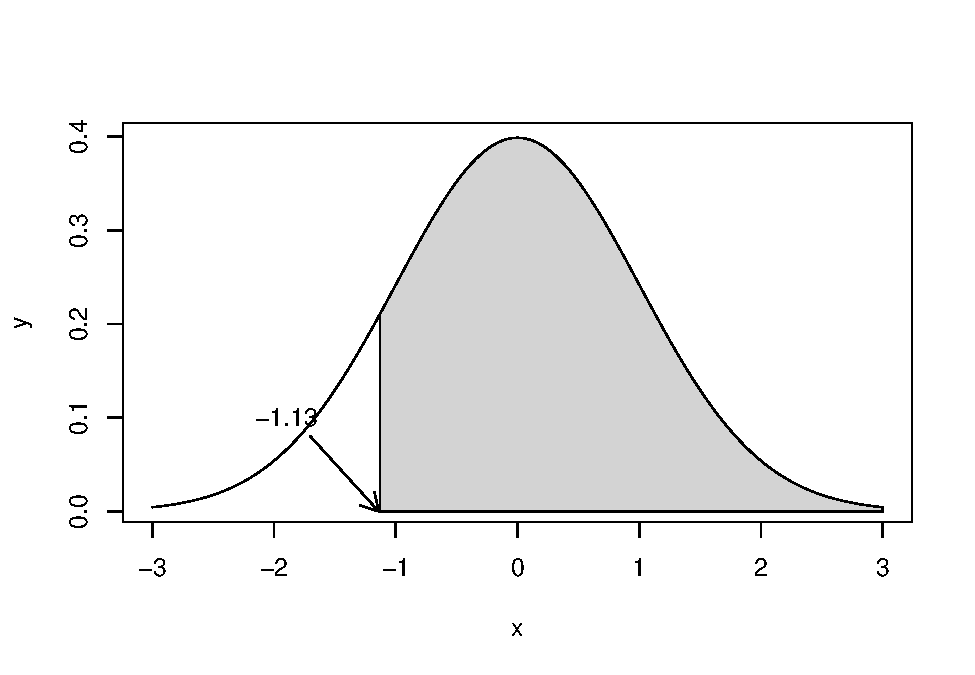
\includegraphics{DATA_606_-_Homework_3_files/figure-latex/unnamed-chunk-1-1.pdf}

\begin{Shaded}
\begin{Highlighting}[]
\DecValTok{1}\NormalTok{-}\KeywordTok{pnorm}\NormalTok{(-}\FloatTok{1.13}\NormalTok{)}
\end{Highlighting}
\end{Shaded}

\begin{verbatim}
## [1] 0.8707619
\end{verbatim}

\begin{enumerate}
\def\labelenumi{(\alph{enumi})}
\setcounter{enumi}{1}
\item
\end{enumerate}

\begin{Shaded}
\begin{Highlighting}[]
\NormalTok{x=}\KeywordTok{seq}\NormalTok{(-}\DecValTok{3}\NormalTok{,}\DecValTok{3}\NormalTok{,}\DataTypeTok{length=}\DecValTok{500}\NormalTok{)}
\NormalTok{y=}\KeywordTok{dnorm}\NormalTok{(x,}\DataTypeTok{mean=}\DecValTok{0}\NormalTok{,}\DataTypeTok{sd=}\DecValTok{1}\NormalTok{)}
\KeywordTok{plot}\NormalTok{(x,y,}\DataTypeTok{type=}\StringTok{"l"}\NormalTok{)}
\NormalTok{x=}\KeywordTok{seq}\NormalTok{(-}\DecValTok{3}\NormalTok{,}\FloatTok{0.18}\NormalTok{,}\DataTypeTok{length=}\DecValTok{100}\NormalTok{)}
\NormalTok{y=}\KeywordTok{dnorm}\NormalTok{(x,}\DataTypeTok{mean=}\DecValTok{0}\NormalTok{,}\DataTypeTok{sd=}\DecValTok{1}\NormalTok{)}
\KeywordTok{polygon}\NormalTok{(}\KeywordTok{c}\NormalTok{(-}\DecValTok{3}\NormalTok{,x,}\FloatTok{0.18}\NormalTok{),}\KeywordTok{c}\NormalTok{(}\DecValTok{0}\NormalTok{,y,}\DecValTok{0}\NormalTok{),}\DataTypeTok{col=}\StringTok{"lightgrey"}\NormalTok{)}
\KeywordTok{arrows}\NormalTok{(}\FloatTok{0.6}\NormalTok{,}\FloatTok{0.08}\NormalTok{,}\FloatTok{0.19}\NormalTok{,}\FloatTok{0.0}\NormalTok{,}\DataTypeTok{length=}\NormalTok{.}\DecValTok{13}\NormalTok{)}
\KeywordTok{text}\NormalTok{(}\FloatTok{0.6}\NormalTok{,}\FloatTok{0.1}\NormalTok{,}\StringTok{"0.18"}\NormalTok{)}
\end{Highlighting}
\end{Shaded}

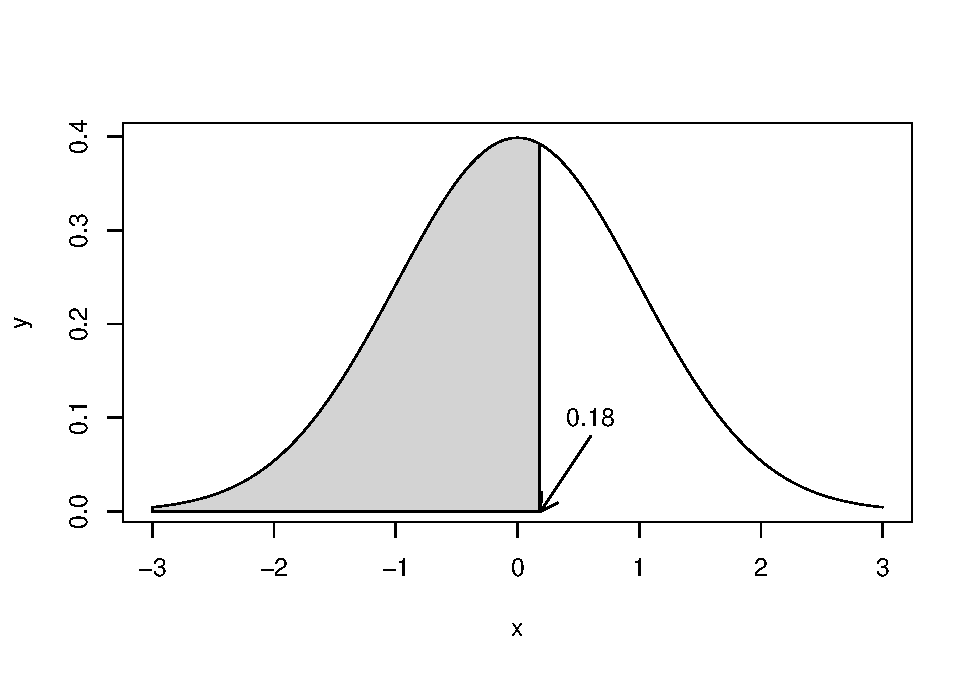
\includegraphics{DATA_606_-_Homework_3_files/figure-latex/unnamed-chunk-2-1.pdf}

\begin{Shaded}
\begin{Highlighting}[]
\KeywordTok{pnorm}\NormalTok{(}\FloatTok{0.18}\NormalTok{)}
\end{Highlighting}
\end{Shaded}

\begin{verbatim}
## [1] 0.5714237
\end{verbatim}

\begin{enumerate}
\def\labelenumi{(\alph{enumi})}
\setcounter{enumi}{2}
\item
\end{enumerate}

\begin{Shaded}
\begin{Highlighting}[]
\NormalTok{x=}\KeywordTok{seq}\NormalTok{(-}\DecValTok{3}\NormalTok{,}\DecValTok{10}\NormalTok{,}\DataTypeTok{length=}\DecValTok{500}\NormalTok{)}
\NormalTok{y=}\KeywordTok{dnorm}\NormalTok{(x,}\DataTypeTok{mean=}\DecValTok{0}\NormalTok{,}\DataTypeTok{sd=}\DecValTok{1}\NormalTok{)}
\KeywordTok{plot}\NormalTok{(x,y,}\DataTypeTok{type=}\StringTok{"l"}\NormalTok{)}
\NormalTok{x=}\KeywordTok{seq}\NormalTok{(}\DecValTok{8}\NormalTok{,}\DecValTok{10}\NormalTok{,}\DataTypeTok{length=}\DecValTok{100}\NormalTok{)}
\NormalTok{y=}\KeywordTok{dnorm}\NormalTok{(x,}\DataTypeTok{mean=}\DecValTok{0}\NormalTok{,}\DataTypeTok{sd=}\DecValTok{1}\NormalTok{)}
\KeywordTok{polygon}\NormalTok{(}\KeywordTok{c}\NormalTok{(}\DecValTok{8}\NormalTok{,x,}\DecValTok{10}\NormalTok{),}\KeywordTok{c}\NormalTok{(}\DecValTok{0}\NormalTok{,y,}\DecValTok{0}\NormalTok{),}\DataTypeTok{col=}\StringTok{"lightgrey"}\NormalTok{)}
\end{Highlighting}
\end{Shaded}

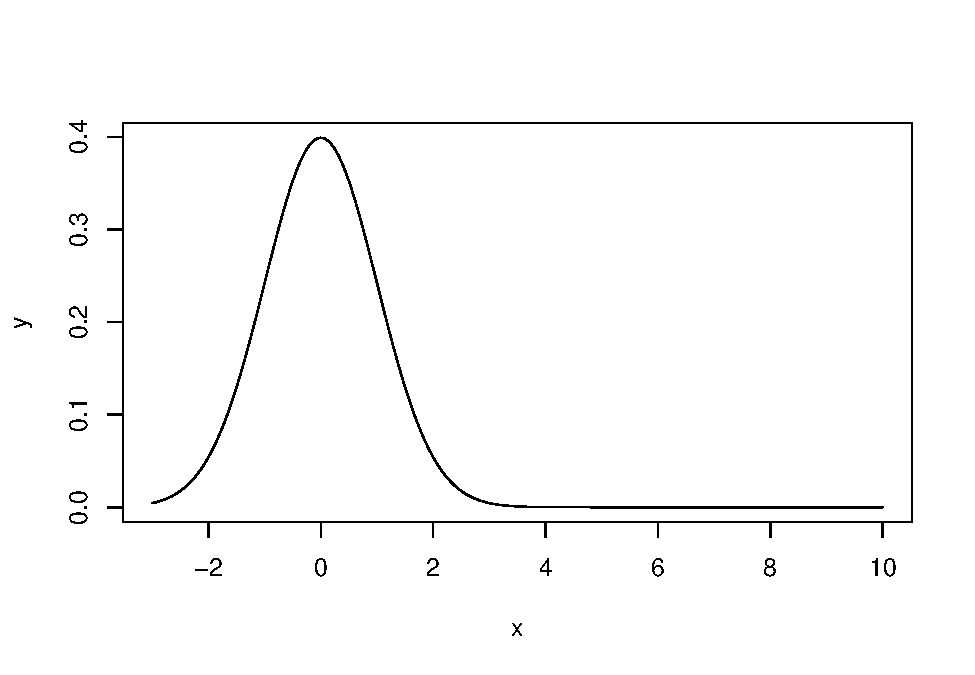
\includegraphics{DATA_606_-_Homework_3_files/figure-latex/unnamed-chunk-3-1.pdf}

\begin{Shaded}
\begin{Highlighting}[]
\DecValTok{1} \NormalTok{-}\StringTok{ }\KeywordTok{pnorm}\NormalTok{(}\DecValTok{8}\NormalTok{)}
\end{Highlighting}
\end{Shaded}

\begin{verbatim}
## [1] 6.661338e-16
\end{verbatim}

\begin{verbatim}
This is an extreme example, so it barely shows on the graph.
\end{verbatim}

\begin{enumerate}
\def\labelenumi{(\alph{enumi})}
\setcounter{enumi}{3}
\item
\end{enumerate}

\begin{Shaded}
\begin{Highlighting}[]
\NormalTok{x=}\KeywordTok{seq}\NormalTok{(-}\DecValTok{3}\NormalTok{,}\DecValTok{3}\NormalTok{,}\DataTypeTok{length=}\DecValTok{500}\NormalTok{)}
\NormalTok{y=}\KeywordTok{dnorm}\NormalTok{(x,}\DataTypeTok{mean=}\DecValTok{0}\NormalTok{,}\DataTypeTok{sd=}\DecValTok{1}\NormalTok{)}
\KeywordTok{plot}\NormalTok{(x,y,}\DataTypeTok{type=}\StringTok{"l"}\NormalTok{)}
\NormalTok{x=}\KeywordTok{seq}\NormalTok{(-}\FloatTok{0.5}\NormalTok{,}\FloatTok{0.5}\NormalTok{,}\DataTypeTok{length=}\DecValTok{100}\NormalTok{)}
\NormalTok{y=}\KeywordTok{dnorm}\NormalTok{(x,}\DataTypeTok{mean=}\DecValTok{0}\NormalTok{,}\DataTypeTok{sd=}\DecValTok{1}\NormalTok{)}
\KeywordTok{polygon}\NormalTok{(}\KeywordTok{c}\NormalTok{(-}\FloatTok{0.5}\NormalTok{,x,}\FloatTok{0.5}\NormalTok{),}\KeywordTok{c}\NormalTok{(}\DecValTok{0}\NormalTok{,y,}\DecValTok{0}\NormalTok{),}\DataTypeTok{col=}\StringTok{"lightgrey"}\NormalTok{)}
\end{Highlighting}
\end{Shaded}

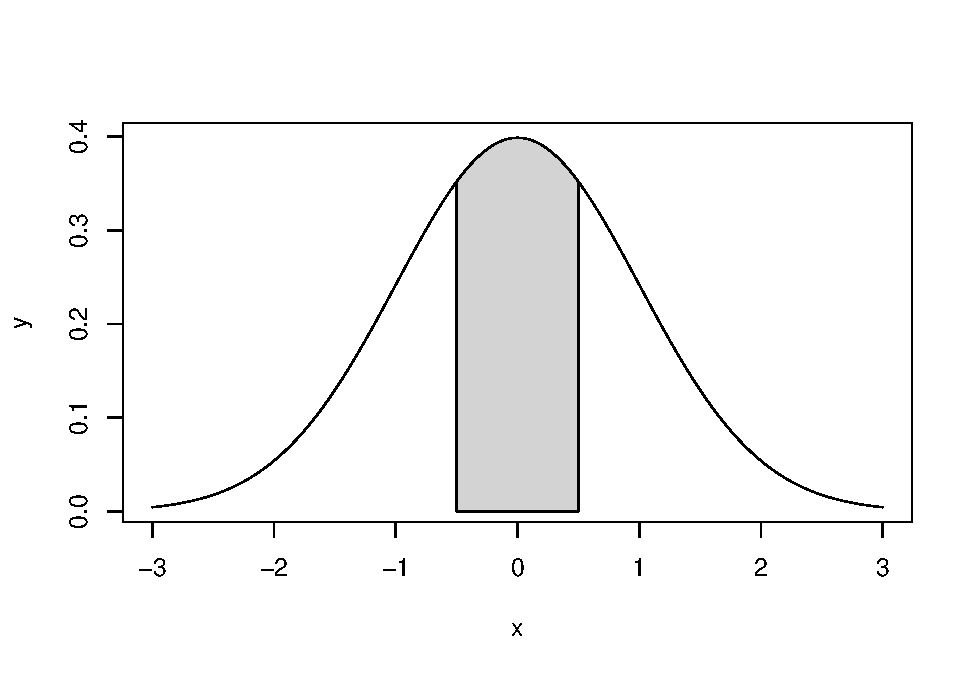
\includegraphics{DATA_606_-_Homework_3_files/figure-latex/unnamed-chunk-4-1.pdf}

\begin{Shaded}
\begin{Highlighting}[]
\KeywordTok{pnorm}\NormalTok{(}\FloatTok{0.5}\NormalTok{)}
\end{Highlighting}
\end{Shaded}

\begin{verbatim}
## [1] 0.6914625
\end{verbatim}

\begin{Shaded}
\begin{Highlighting}[]
\KeywordTok{pnorm}\NormalTok{(-}\FloatTok{0.5}\NormalTok{)}
\end{Highlighting}
\end{Shaded}

\begin{verbatim}
## [1] 0.3085375
\end{verbatim}

\subsection{3.4 Triathlon times, Part I}\label{triathlon-times-part-i}

In triathlons, it is common for racers to be placed into age and gender
groups. Friends Leo and Mary both completed the Hermosa Beach Triathlon,
where Leo competed in the Men, Ages 30 - 34 group while Mary competed in
the Women, Ages 25 - 29 group. Leo completed the race in 1:22:28 (4948
seconds), while Mary completed the race in 1:31:53 (5513 seconds).
Obviously Leo finished faster, but they are curious about how they did
within their respective groups. Can you help them? Here is some
information on the performance of their groups:

\begin{itemize}
\item
  The finishing times of the Men, Ages 30 - 34 group has a mean of 4313
  seconds with a standard deviation of 583 seconds.
\item
  The finishing times of the Women, Ages 25 - 29 group has a mean of
  5261 seconds with a standard deviation of 807 seconds.
\item
  The distributions of finishing times for both groups are approximately
  Normal. Remember: a better performance corresponds to a faster finish.
\end{itemize}

\begin{enumerate}
\def\labelenumi{(\alph{enumi})}
\tightlist
\item
  Write down the short-hand for these two normal distributions.
\item
  What are the Z-scores for Leo's and Mary's finishing times? What do
  these Z-scores tell you?
\item
  Did Leo or Mary rank better in their respective groups? Explain your
  reasoning.
\item
  What percent of the triathletes did Leo finish faster than in his
  group?
\item
  What percent of the triathletes did Mary finish faster than in her
  group?
\item
  If the distributions of finishing times are not nearly normal, would
  your answers to parts (b) - (e) change? Explain your reasoning.
\end{enumerate}

Solutions:\\
(a) For the men's group: \(N(\mu = 4313, \sigma = 583)\). For the
women's group: \(N(\mu = 5261, \sigma = 807)\).\\
(b) \(Z = \frac{x=\mu}{\sigma}.\)\\
\(Z_L = \frac{4948-4313}{583} = 1.0892\).
\(Z_M = \frac{5513-5261}{807} = 0.3123\).\\
Leo scored 1.09 standard deviations above the mean, while Mary scored
0.31 standard deviations above the mean, each in their respective
groups.\\
(c) Since Mary's z-score is smaller, it mean's she finished closer to
the mean of her group, so she did better in her respective group.\\
(d) \(P(Z_L > 1.0892)\)

\begin{Shaded}
\begin{Highlighting}[]
\DecValTok{1} \NormalTok{-}\StringTok{ }\KeywordTok{pnorm}\NormalTok{(}\FloatTok{1.0892}\NormalTok{)}
\end{Highlighting}
\end{Shaded}

\begin{verbatim}
## [1] 0.1380328
\end{verbatim}

\begin{verbatim}
~0.86 finished faster than leo, which means Leo finished faster than 1 - ~0.86 = ~0.13.
\end{verbatim}

\begin{enumerate}
\def\labelenumi{(\alph{enumi})}
\setcounter{enumi}{4}
\tightlist
\item
  \(P(Z_M > 0.3123)\)
\end{enumerate}

\begin{Shaded}
\begin{Highlighting}[]
\DecValTok{1} \NormalTok{-}\StringTok{ }\KeywordTok{pnorm}\NormalTok{(}\FloatTok{0.3123}\NormalTok{)}
\end{Highlighting}
\end{Shaded}

\begin{verbatim}
## [1] 0.3774063
\end{verbatim}

\begin{verbatim}
Using the same method as (d), we find that Mary was faster than 0.37 of her group.
\end{verbatim}

\begin{enumerate}
\def\labelenumi{(\alph{enumi})}
\setcounter{enumi}{5}
\tightlist
\item
  The Z-scores would remain the same, since we can calculate them in
  non-normal distributions. The rest of the answers would change,
  though, because we can't calculate probabilities and percentiles using
  Z-scores for non-normal distributions.
\end{enumerate}

\subsection{3.18 Heights of female college
students.}\label{heights-of-female-college-students.}

\begin{enumerate}
\def\labelenumi{(\alph{enumi})}
\tightlist
\item
  The mean height is 61.52 inches with a standard deviation of 4.58
  inches. Use this information to determine if the heights approximately
  follow the 68-95-99.7\% Rule.
\item
  Do these data appear to follow a normal distribution? Explain your
  reasoning using the graphs provided below.
\end{enumerate}

Solutions:\\
(a)

\begin{verbatim}
The 68-95-99.7% Rule states that for normal distributions,68% of the data fall within 1 standard deviation of the mean, 95% within 2 sd, and 99.7 within 3 sd.
To verify, let's input the data:
\end{verbatim}

\begin{Shaded}
\begin{Highlighting}[]
\NormalTok{heights <-}\StringTok{ }\KeywordTok{c}\NormalTok{(}\DecValTok{54}\NormalTok{,}\DecValTok{55}\NormalTok{,}\DecValTok{56}\NormalTok{,}\DecValTok{56}\NormalTok{,}\DecValTok{57}\NormalTok{,}\DecValTok{58}\NormalTok{,}\DecValTok{58}\NormalTok{,}\DecValTok{59}\NormalTok{,}\DecValTok{60}\NormalTok{,}\DecValTok{60}\NormalTok{,}\DecValTok{60}\NormalTok{,}\DecValTok{61}\NormalTok{,}\DecValTok{61}\NormalTok{,}\DecValTok{62}\NormalTok{,}\DecValTok{62}\NormalTok{,}\DecValTok{63}\NormalTok{,}\DecValTok{63}\NormalTok{,}\DecValTok{63}\NormalTok{,}\DecValTok{64}\NormalTok{,}\DecValTok{65}\NormalTok{,}\DecValTok{65}\NormalTok{,}\DecValTok{67}\NormalTok{,}\DecValTok{67}\NormalTok{,}\DecValTok{69}\NormalTok{,}\DecValTok{73}\NormalTok{)}
\NormalTok{mean <-}\StringTok{ }\FloatTok{61.52}
\NormalTok{sd <-}\StringTok{ }\FloatTok{4.58}
\end{Highlighting}
\end{Shaded}

\begin{Shaded}
\begin{Highlighting}[]
\CommentTok{# for 68%:}
\NormalTok{x1 <-}\StringTok{ }\NormalTok{mean -}\StringTok{ }\NormalTok{sd}
\NormalTok{x2 <-}\StringTok{ }\NormalTok{mean +}\StringTok{ }\NormalTok{sd}
\NormalTok{v1 <-}\StringTok{ }\KeywordTok{pnorm}\NormalTok{(x2,mean,sd) -}\StringTok{ }\KeywordTok{pnorm}\NormalTok{(x1,mean,sd)}
\NormalTok{v1}
\end{Highlighting}
\end{Shaded}

\begin{verbatim}
## [1] 0.6826895
\end{verbatim}

\begin{Shaded}
\begin{Highlighting}[]
\CommentTok{# for 95%:}
\NormalTok{y1 <-}\StringTok{ }\NormalTok{mean -}\StringTok{ }\DecValTok{2}\NormalTok{*sd}
\NormalTok{y2 <-}\StringTok{ }\NormalTok{mean +}\StringTok{ }\DecValTok{2}\NormalTok{*sd}
\NormalTok{v2 <-}\StringTok{ }\KeywordTok{pnorm}\NormalTok{(y2,mean,sd) -}\StringTok{ }\KeywordTok{pnorm}\NormalTok{(y1,mean,sd)}
\NormalTok{v2}
\end{Highlighting}
\end{Shaded}

\begin{verbatim}
## [1] 0.9544997
\end{verbatim}

\begin{Shaded}
\begin{Highlighting}[]
\CommentTok{# for 99.7%:}
\NormalTok{z1 <-}\StringTok{ }\NormalTok{mean -}\StringTok{ }\DecValTok{3}\NormalTok{*sd}
\NormalTok{z2 <-}\StringTok{ }\NormalTok{mean +}\StringTok{ }\DecValTok{3}\NormalTok{*sd}
\NormalTok{z3 <-}\StringTok{ }\KeywordTok{pnorm}\NormalTok{(z2,mean,sd) -}\StringTok{ }\KeywordTok{pnorm}\NormalTok{(z1,mean,sd)}
\NormalTok{z3}
\end{Highlighting}
\end{Shaded}

\begin{verbatim}
## [1] 0.9973002
\end{verbatim}

\begin{verbatim}
We can see that the heights adhere to the 68-95-99.7 rule almost perfectly.
\end{verbatim}

\begin{enumerate}
\def\labelenumi{(\alph{enumi})}
\setcounter{enumi}{1}
\item
\begin{verbatim}
The histogram does closely fit the normal curve, and the normal probability plot is almost perfectly straight (aside from a few outliers), so we can conclude that the heights appear to follow the normal distribution.
\end{verbatim}
\end{enumerate}

\subsection{3.22 Defective Rate}\label{defective-rate}

A machine that produces a special type of transistor (a component of
computers) has a 2\% defective rate. The production is considered a
random process where each transistor is independent of the others.\\
(a) What is the probability that the 10th transistor produced is the
first with a defect?\\
(b) What is the probability that the machine produces no defective
transistors in a batch of 100?\\
(c) On average, how many transistors would you expect to be produced
before the first with a defect? What is the standard deviation?\\
(d) Another machine that also produces transistors has a 5\% defective
rate where each transistor is produced independent of the others. On
average how many transistors would you expect to be produced with this
machine before the first with a defect? What is the standard
deviation?\\
(e) Based on your answers to parts (c) and (d), how does increasing the
probability of an event affect the mean and standard deviation of the
wait time until success?

Solutions:\\
(a) Since we're trying to find the \emph{first} instance that satisfies
our condition, we're dealing with a geometric distribution. The formula
for Geometric distribution is: \((1-p)^{n-1}\cdot p\).\\
Let \(p = 0.02\) be the probability that the transistor is defective.
Then, \((1-p) = 0.98\).\\
\((0.98)^{9}\cdot 0.02 = 0.0167\).\\
(b) Since \(p\) is defined as the transistor being defective, we want
the first 100 transistors to be working, i.e. \((1-p)\).\\
\((1-p)^{100} = (0.98)^{100} = 0.1326\).\\
(c) For Geometric distribution, the mean (expected value) is
\(\frac{1}{p}\), and the standard deviation is
\(\sqrt{\frac{1-p}{p^2}}\).\\
\(\mu = \frac{1}{0.02} = 50 \qquad \sigma = \sqrt{\frac{0.98}{(0.02)^2}} = 49.4975\).\\
So we can expect to produce 50 working transistors before making a
defective one, with a standard deviation of 49.4975.\\
(d) Using the same formulas as in (c), we get:\\
\(\mu = \frac{1}{0.05} = 20, \qquad \sigma = \sqrt{\frac{0.95}{(0.05)^2}} = 19.4936\).\\
For this machine, we can expect to produce 20 working transistors before
making a defective one, with a standard deviation of 19.4936.\\
(e) If we increase the probability of producing a defective transistor,
we can expect to produce fewer working ones before making our first
defective one. Similarly, our standard deviation will shrink, as well.

\subsection{3.38 Male Children}\label{male-children}

While it is often assumed that the probabilities of having a boy or a
girl are the same, the actual probability of having a boy is slightly
higher at 0.51. Suppose a couple plans to have 3 kids.\\
(a) Use the binomial model to calculate the probability that two of them
will be boys.\\
(b) Write out all possible orderings of 3 children, 2 of whom are boys.
Use these scenarios to calculate the same probability from part (a) but
using the addition rule for disjoint outcomes.\\
Confirm that your answers from parts (a) and (b) match.\\
(c) If we wanted to calculate the probability that a couple who plans to
have 8 kids will have 3 boys, briefly describe why the approach from
part (b) would be more tedious than the approach from part (a).\\
Solutions:\\
(a) The general formula for the binomial distribution is:
\(\binom{n}{k}p^k(1-p)^{n-k}\).
\(\binom{3}{2}(0.51)^{2}\cdot(0.49)^{1} = 0.382347.\)\\
(b) There are three possible scenarios, with their corresponding
probabilites:\\

\begin{itemize}
\tightlist
\item
  boy, boy, girl \(\qquad 0.51\times0.51\times0.49\)
\item
  boy, girl, boy \(\qquad 0.51\times0.49\times0.51\)
\item
  girl, boy, boy \(\qquad 0.49\times0.51\times0.51\)
\end{itemize}

Since they are disjoint events, we can sum the probabilities:

\begin{Shaded}
\begin{Highlighting}[]
\NormalTok{x1 <-}\StringTok{ }\FloatTok{0.51}\NormalTok{*}\FloatTok{0.51}\NormalTok{*}\FloatTok{0.49}
\NormalTok{x2 <-}\StringTok{ }\FloatTok{0.51}\NormalTok{*}\FloatTok{0.49}\NormalTok{*}\FloatTok{0.51}
\NormalTok{x3 <-}\StringTok{ }\FloatTok{0.49}\NormalTok{*}\FloatTok{0.51}\NormalTok{*}\FloatTok{0.51}
\NormalTok{s <-}\StringTok{ }\KeywordTok{sum}\NormalTok{(x1,x2,x3)}
\NormalTok{s}
\end{Highlighting}
\end{Shaded}

\begin{verbatim}
## [1] 0.382347
\end{verbatim}

\begin{enumerate}
\def\labelenumi{(\alph{enumi})}
\setcounter{enumi}{2}
\tightlist
\item
  If we would use the method from (b), we'd have to map out each
  possible permutation (\(\binom{8}{3} = 56\)), which is a lot of extra,
  unnecessary work.
\end{enumerate}

\subsection{3.42 Serving in Volleyball}\label{serving-in-volleyball}

A not-so-skilled volleyball player has a 15\% chance of making the
serve, which involves hitting the ball so it passes over the net on a
trajectory such that it will land in the opposing team's court. Suppose
that her serves are independent of each other.\\
(a) What is the probability that on the 10th try she will make her 3rd
successful serve?\\
(b) Suppose she has made two successful serves in nine attempts. What is
the probability that her 10th serve will be successful?\\
(c) Even though parts (a) and (b) discuss the same scenario, the
probabilities you calculated should be different. Can you explain the
reason for this discrepancy?

Solutions:\\
(a) We're dealing with a negative binomial distribution. The general
formula is: \(\binom{n-1}{k-1}\cdot p^k\cdot(1-p)^{n-k}\).\\
\(\binom{9}{2}(0.15)^{3}(0.85)^{7} = 0.039\).\\
(b) Since these events are independent, the success in previous attempts
has no effect on subsequent serves. Therefore, the probability of
success is still 0.15.\\
(c) For (a), we're looking for the probability of the kth success in the
nth trial, so we have to calculate the negative binomial. In (b), we're
not concerned with previous successes, just the probability of success
in a single scenario, so it's just \(p\).


\end{document}
